\documentclass[a4paper,12pt]{article}
%%%%%%%%%%%%%%%%%%%%%%%%%%%%%%%%%%%%%%%%%%%%%%%%%%%%%%%%%%%%%%%%%%%%%%%%%%%%%%%%%%%%%%%%%%%%%%%%%%%%%%%%%%%%%%%%%%%%%%%%%%%%%%%%%%%%%%%%%%%%%%%%%%%%%%%%%%%%%%%%%%%%%%%%%%%%%%%%%%%%%%%%%%%%%%%%%%%%%%%%%%%%%%%%%%%%%%%%%%%%%%%%%%%%%%%%%%%%%%%%%%%%%%%%%%%%
\usepackage{eurosym}
\usepackage{vmargin}
\usepackage{amsmath}
\usepackage{graphics}
\usepackage{epsfig}
\usepackage{subfigure}
\usepackage{fancyhdr}
\usepackage{listings}
\usepackage{framed}
\usepackage{graphicx}
\usepackage{amsmath}
\usepackage{chngpage}
%\usepackage{bigints}

\setcounter{MaxMatrixCols}{10}

\begin{document}
\Large
\section*{Using Palettes}
\begin{itemize}
\item Palettes are sequences (lists or tuples) of RGB(A) hex strings that define a colormap and be can set as the palette attribute of all chart types from \texttt{bokeh.charts} and as the color attribute of many plot objects from \texttt{bokeh.plotting}. 
\item Bokeh offers many of the standard Brewer palettes, which can be imported from the \texttt{bokeh.palettes} module. 
\item For example, importing “\texttt{Spectral6}” gives a six element list of RBG(A) hex strings from the Brewer “Spectral” colormap.
\end{itemize}

\begin{figure}[h!]
\centering
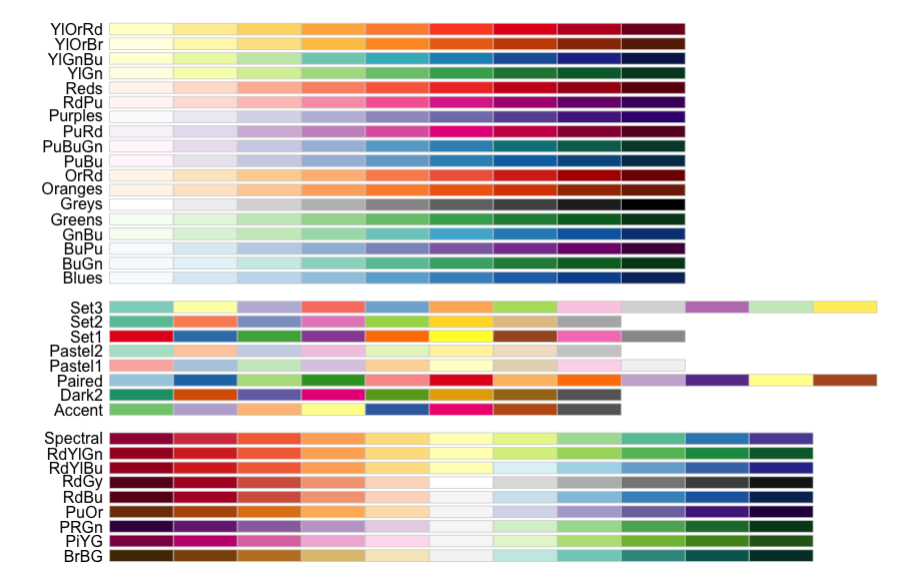
\includegraphics[width=1.2\linewidth]{images/04-pallettes-brewer}

\end{figure}

\newpage

{
	\large
\begin{framed}
\begin{verbatim}
>>> from bokeh.palettes import Spectral6
>>> Spectral6
[ '#3288bd', '#99d594', '#e6f598', 
  '#fee08b', '#fc8d59', '#d53e4f']

\end{verbatim}
\end{framed}
}
\begin{itemize}
\item All of the standard palettes included in bokeh can be found at Standard Palettes.
\item  Custom palettes can be made by creating sequences of RGB(A) hex strings.
\end{itemize}

%============================================= %

\subsection*{Colourblind Friendly Palettes} The default Palettes, that are used by high level charts,  contain red and green are inappropriate for any colourblind users.
{
	\large
	\begin{framed}
		\begin{verbatim}
		
from bokeh.palettes import brewer
palette = brewer["Blues"][3]
\end{verbatim}
\end{framed}
}
pass palette into chart call e.g.

{
	\large
	\begin{framed}
		\begin{verbatim}
		
bar = Bar(medals, countries, title="grouped, dict_input", 
xlabel="countries", 
ylabel="medals", 
legend=True, width=800, height=600, 
notebook=True, palette=palette)
\end{verbatim}
\end{framed}
}
\noindent Palette can actually be a list of any values you want, but there's inbuilt palettes listed in the Bokeh documentation. %http://bokeh.pydata.org/en/latest/docs/reference/palettes.html


\end{document}